
\marginpar{\textcolor{red}{Vorlesung 3}}

\begin{deff}
F\"ur ein Mengensystem $\mathcal E\subseteq \mathcal P(\Omega)$ hei\ss t
	\[ d(\mathcal{E}) = \bigcap\limits_{\substack{\cE \subseteq \cD,\\ \cD \text{ Dynk.-S.}}} \! \! \! \! \! \! \! \cD \] das $\cE$ erzeugtes Dynkin-System. Dass $d(\mathcal E)$ das kleinste Dynkin-System ist das $\mathcal E$ enh\"alt, zeigt man genauso wie f\"ur $\sigma$-Algebren.
\end{deff}

\begin{satz}[Hauptsatz für Dynkin-Systeme] \label{Hauptsatz}
	Ist $\cE \subseteq \cP (\Omega)$ $\cap$-stabil, so gilt $d(\cE) = \sigma(\cE)$.
\end{satz}

\begin{proof}
	Die Richtung $d(\cE) \subseteq \sigma(\cE)$ folgt sofort, denn jede $\sigma$-Algebra ist auch immer ein Dynkin-System, folglich gilt \[d(\cE) = \bigcap\limits_{\substack{\cE \subseteq \cD,\\ \cD \text{ Dynk.-S.}}} \! \! \! \! \! \! \! \cD \,\,\subseteq \,\,\bigcap\limits_{\substack{\mathcal E \subseteq \cB, \\ \cB \: \sigma \text{-Alg.}}} \! \! \! \! \cB= \sigma(\cE) .\]
	Für die Richtung $\sigma(\cE) \subseteq d(\cE)$ nehmen wir an, dass $d(\cE)$ $\cap$-stabil ist. Denn in diesem Fall folgt nach \ref{dschnitt}, dass $d(\cE)$ eine $\sigma$-Algebra ist. Weil dann aber $\cE \subseteq d(\cE)$ gilt, muss die kleinste $\sigma$-Algebra (was gerade $\sigma(\cE)$ ist) in $d(\cE)$ sein. Wir müssen also nur noch zeigen, dass $d(\cE)$ $\cap$-stabil, wenn $\mathcal E$ $\cap$-stabil ist:
	\begin{itemize}
		\item[(a)] \label{cD_D} Definiere dazu zun\"achst \[\cD_D = \{ \cA \in \cP(\Omega): A \cap D \in d(\cE) \}\] für beliebige $D \in d(\cE)$. Wir zeigen zun\"achst, dass $\cD_D$ ein Dynkin-System ist:
		\begin{enumerate}[label=(\roman*)]
			\item Weil per Annahme $D \in d(\cE)$ und $D =  \Omega \cap D$ gilt, ist $\Omega \in \cD_D$.
			\item Sei $A \in \cD_D$. Damit auch $A^C \in \cD_D$ gilt, zeigen wir $A^C \cap D \in d(\cE)$. Da Dynkin-Systeme abgeschlossen bezüglich disjunkter Vereinigung sind, folgt \[ A^C \cap D = (A \cup D^C)^C = (\underbrace{(A \cap D)}_{\in d(\cE)} \cupdot D^C)^C \in d(\cE). \]
			\item Seien $A_1, A_2,... \in \cD_D$ paarweise disjunkt, dann gilt \[ 
			\bigcupdot\limits_{n=1}^{\infty} A_n \cap D = \bigcupdot\limits_{n=1}^{\infty} \underbrace{(A_n \cap D)}_{\in d(\cE)} \in d(\cE). \]
		\end{enumerate}
		\item[(b)] Es gilt $d(\cE) \subseteq \cD_D$  für alle $D \in \cE$. Warum? Sei $A \in \cE$, so ist $A \cap D \in \cE$, weil $\cE$ nach Annahme $\cap$-stabil ist. Damit ist $A \in \cD_D$ und folglich $\cE \subseteq \cD_D$. Dann gilt aber auch $d(\cE) \subseteq d(\cD_D) \overset{(a)}{=} \cD_D$ weil das von einem Dynkin-System $\mathcal D$ erzeugte Dynkin-System gerade $\mathcal D$ ist. 
		\item[(c)]Des Weiteren gilt wegen (b) auch $\cE \subseteq \cD_D$  für alle $D \in d(\cE)$, d.h. $D\cap E\in d(\mathcal E)$ f\"ur alle $E \in \mathcal E$.
				\item[(d)] Aus (c) und (a) folgt $d(\cE) \subseteq d(\cD_D)= \cD_D$ für alle $D \in d(\cE)$. Das ist wegen Definition von $\cD_D$ gerade die $\cap $-Stabilit\"at von $d(\mathcal E)$.
	\end{itemize}
\end{proof}
Nun kommen wir zu der wesentlichen Anwendung von Dynkin-Systemen. Mit Dynkin-Systemen k\"onnen wir ganz einfach zeigen, dass die Gleichheit von Ma\ss en schon aus der Gleichheit auf einem schnittstabilen Erzeuger folgt. Wenn wir an die wahnsinnig gro\ss e Borel-$\sigma$-Algebra denken, macht das ganze schnell Sinn. Es reicht n\"amlich die Gleichheit auf allen Intervallen zu zeigen, statt auf allen Borelmengen.
\begin{korollar}\label{Dynkin-Folgerung}
	Sei $(\Omega, \cA)$ ein messbarer Raum und $\cE$ ein $\cap$-stabiler Erzeuger von $\cA$. Sind $\mu_1,\mu_2$ endliche Maße auf $\cA$ und es gelten
	\begin{itemize}
		\item $\mu_1(\Omega)=\mu_2(\Omega)$,
		\item $\mu_1(A) = \mu_2(A)$ für alle $A \in \cE$, 
	\end{itemize}
	so gilt $\mu_1(A) = \mu_2(A)$ für alle $A \in \cA$, \mbox{d. h.} $\mu_1 = \mu_2$.
\end{korollar}

\begin{proof}
	Wir haben schon gezeigt, dass
	\[ \cM = \{ A \in \cA \! : \mu_1(A) = \mu_2(A) \} \] ein Dynkin-System ist. Nach Annahme ist $\cE \subseteq \cM$. Weil $\cM$ ein Dynkin-System ist, gilt $d(\cE) \subseteq d(\cM) = \cM \subseteq \cA$. Weil nach Annahme $\cE$ $\cap$-stabil ist, gilt nach dem Hauptsatz \"uber Dynkin-Systeme $\sigma(\cE) = d(\cE)$. Nach Annahme ist aber $\sigma(\cE) = \cA$. Alles zusammen ergibt \[ \cA = \sigma(\cE) = d(\cE) \subseteq d(\cM) = \cM \subseteq \cA. \] Also gilt $\cM = \cA$ und das ist die Aussage des Korollars.
\end{proof}

Wir schauen uns noch einen Trick an, die Endlichkeitsannahme aus Korollar \ref{Dynkin-Folgerung} abzuschw\"achen.
\begin{korollar}[Eindeutigkeitssatz]\label{folg}
	Es sei $(\Omega, \cA)$ ein messbarer Raum, $\cE$ ein $\cap$-stabiler Erzeuger von $\cA$ und $\mu_1,\mu_2$ seien Maße auf $\cA$. Zudem gelten:
	\begin{enumerate}[label=(\roman*)]		
		\item Es gibt eine Folge $(E_n) \subseteq \mathcal A$ mit $E_n \uparrow \Omega$, $n \to \infty$, und $\mu_i(E_n) < \infty$ für alle $n \in \N$, $i = 1,2$.		
		%% Alternativ:
		% \item Es gibt eine Folge $(E_n) \subseteq \cA$ mit $E_n \uparrow \Omega$, $n \to \infty$ und ${{\mu_1(E_n)} \atop {\mu_2(E_n)}} < \infty$ für alle $n\in \N$.
		\item $\mu_1(A) = \mu_2(A)$ für alle $A \in \cE$.
	\end{enumerate}
	Dann gilt $\mu_1 = \mu_2$, \mbox{d. h.} $\mu_1(A) = \mu_2(A)$ für alle $A \in \cA$.
\end{korollar}
Geben wir der genutzten Erweiterung endlicher Ma\ss e einen Namen: 
\begin{deff}
	Ist $(\Omega, \cA, \mu)$ ein Maßraum und es gibt eine Folge $(E_n) \subseteq \cA$ mit $E_n \uparrow \Omega$, $n \to \infty$, und $\mu(E_n) < \infty$ f\"ur alle $n \in \N$, so nennt man $\mu$ ein \textbf{$\sigma$-endliches Maß}.
\end{deff}
Die meisten S\"atze f\"ur endliche Ma\ss e lassen sich mit dem Trick des folgenden Beweises auf $\sigma$-endliche Ma\ss e ausdehen. Beispiele folgen noch.

\begin{proof}[Beweis von \ref{folg}]
Definiere dazu für $A \in \cA$ und $n \in \N$
	\begin{align*}
	&\mu_1^{n}(A) := \mu_1(A\cap E_n),\\
	&\mu_2^{n}(A) := \mu_2(A\cap E_n).
	\end{align*}
	Man rechnet sofort nach, dass auch die $\mu_i^n$ wieder Ma\ss e auf $\mathcal A$ sind. Des Weiteren sind $\mu_1^{n}, \mu_2^{n}$ endlich, weil $\mu_i^{n} (\Omega) = \mu_i(\Omega \cap E_n) = \mu_i(E_n) \overset{\text{Ann.}}{<} \infty$. Nach \ref{Hauptsatz} gilt $\mu_1^{n} = \mu_2^{n}$ für alle $n \in \N$. Nun gilt wegen Stetigkeit von Ma\ss en
	\begin{gather*}
	\mu_1(A) = \mu_1(A \cap \Omega) = \mu_1\Big(A \cap \bigcup\limits_{n=1}^{\infty} E_n\Big) = \mu_1\Big(\bigcup\limits_{n=1}^{\infty} (A\cap E_n)\Big) \overset{\ref{S1}}{=} \lim\limits_{n \to \infty} \mu_1(A\cap E_n) \\ 
	\overset{\text{Def.}}{=} \lim\limits_{n \to \infty} \mu^n_1(A) = \lim\limits_{n \to \infty} \mu^n_2(A) \overset{\text{Def.}}{=}  \lim\limits_{n \to \infty} \mu_2(A\cap E_n) \overset{\ref{S1}}{=} \mu_2\Big(A \cap \bigcup\limits_{n=1}^{\infty} E_n\Big) = \mu_2(A).
	\end{gather*}
\end{proof}
So, endlich ein Beispiel!
\begin{beispiel}
	Sei $\mathbb P$ ein Wahrscheinlichkeitsma\ss{} auf $\cB(\mathbb{R})$. Dann heißt $$F_{\mathbb{P}}(t) := \mathbb{P}((-\infty,t]), \quad t\in \R, $$die \textbf{Verteilungsfunktion} von $\mathbb{P}$. $F_{\mathbb{P}}$ erfüllt folgende Eigenschaften:
	\begin{itemize}
		\item $0 \leq F_{\mathbb{P}} \leq 1$,
		\item $F_{\mathbb{P}}$ ist nicht fallend,
		\item $\lim_{t\to +\infty} F_{\mathbb P}(t)=1$,
		\item $\lim_{t\to -\infty} F_{\mathbb P}(t)=0$.
	\end{itemize}
	Die ersten beiden Eigenschaften folgen aus der Definition von Wahrscheinlichkeitsma\ss es und der Monotonie von Ma\ss en. Die weiteren Eigenschaften folgen aus der Stetigkeit von Ma\ss en. Um die gerade bewiesenen S\"atze anzuwenden zeigen wir folgende Behauptung: $$F_{\mathbb{P}_1}(t) = F_{\mathbb{P}_2}(t) \quad \text{f\"ur alle } t\in \mathbb{R}\quad \Longrightarrow \quad\mathbb{P}_1 = \mathbb{P}_2.$$ Das folgt aus \ref{Dynkin-Folgerung} mit $\cE = \{ (-\infty,t] \! : t\in \mathbb{R} \} \subseteq \cP(\mathbb{R})$. Checken wir dazu die ben\"otigten Eigenschaften:
	\begin{itemize}
		\item $\sigma(\cE) = \cB(\mathbb{R})$ ist aus den \"Ubungen bekannt,
		\item $\cE$ ist $\cap$-stabil, denn $(-\infty,s] \cap (-\infty,t] = (-\infty, \min\{ s,t \}]$, $s,t \in \mathbb{R}$,
		\item $\mathbb{P}_1(A) = \mathbb{P}_2(A)$ f\"ur alle $A \in \cE$ weil das gerade die Verteilungsfunktionen sind.
	\end{itemize}
\end{beispiel}
Genauso beweist man auch die Aussage des n\"achsten Beispiels:
\begin{beispiel}
	Seien $\mu_1, \mu_2$ endliche Maße auf $\cB(\mathbb{R}^d)$ mit einer der folgenden Eigenschaften:
	\begin{align*}
	&\mu_1(Q) = \mu_2(Q) \text{ für alle Quader } Q,\\
	&\mu_1(K) = \mu_2(K) \text{ für alle kompakten Mengen } K,\\
	&\mu_1(O) = \mu_2(O) \text{ für alle offenen Mengen } O,\\
	&\mu_1(A) = \mu_2(A) \text{ für alle abgeschlossenen Mengen } A.\\
	\end{align*}
	Dann gilt $\mu_1 = \mu_2$.
\end{beispiel}

\section{Konstruktion von Maßen}
Gerade haben wir gesehen, dass zwei endliche Ma\ss e auf $\mathcal B(\R)$ schon auf den Intervallen eindeutlich festgelegt sind (sind $\mu_1$, $\mu_2$ gleich auf Intervallen, sind $\mu_1,$ $\mu_2$ gleich auf $\mathcal B(\mathbb R)$). Das ist eine Eindeutigkeitsaussage. Jetzt drehen wir das ganze um und untersuchen Existenzaussagen. Am Ende soll folgendes rauskommen: Wenn wir eine \glqq geeignete Mengenfunktion\grqq{} auf den Intervallen definieren, dann gibt es auch ein passendes Ma\ss{} auf $\mathcal B(\R)$. Dazu brauchen wir einiges an Handwerkszeugs.
\begin{deff}
	$\cS \subseteq \cP(\Omega)$ heißt \textbf{Semiring}, falls
	\begin{enumerate}[label=(\roman*)]
		\item $\emptyset \in \cS$
		\item $A,B \in \cS \Rightarrow A\cap B \in \cS$, also ist $\mathcal S$ \enquote{$\cap$-stabil}
		\item \label{semiring drittens} $A,B \in \cS$, $B \subseteq A \Rightarrow$ es gibt paarweise disjunkte Mengen $C_1,...,C_n \in \cS$ mit \[ A \backslash B = \bigcupdot\limits_{k=1}^{n} C_k. \]
	\end{enumerate}
\end{deff}
Die Definition ist etwas komisch, verallgemeinert aber einfach nur das folgendes Beispiel, dass wir immer im Kopf halten und sp\"ater auch haupts\"achlich nutzen:
\begin{beispiel1}
	$\cQ := \{ Q \subseteq \mathbb{R}^d \! : Q \text{ Quader} \}$ ist ein Semiring. Checken wir anschaulich die definierenden Eigenschaften, vern\"unftige Argumente haben wir in Analysis II gesehen (Stichwort Quaderwahnsinn):
	\begin{enumerate}[label=(\roman*)]
		\item $\emptyset \in \cQ$ weil $\emptyset = (a_1,a_1)\times ... \times (a_d,a_d)$ f\"ur beliebige $a_1, ..., a_d\in\R$.
		\item \abs 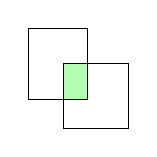
\begin{tikzpicture}[scale=0.75]
		\draw (0,0) rectangle (1,1.2);
		\draw (0.6,0.6) rectangle (1.7,-0.5);
		\draw[fill=green!30] (0.6,0.6) rectangle (1,0);
		\end{tikzpicture}
		\item \abs 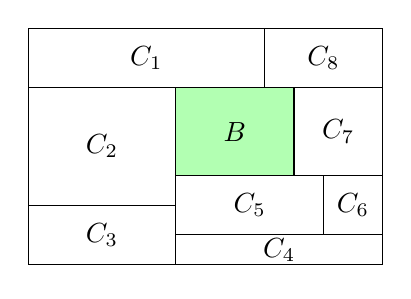
\begin{tikzpicture}[scale=0.75]
		\draw (0,0) rectangle (6,4);
		\draw[fill=green!30] (2.5,1.5) rectangle (4.5,3);		
		\draw (3.5, 2.25) node {$B$};
		\draw (0,4) rectangle (4,3);		
		\draw (2, 3.5) node {$C_1$};
		\draw (0,3) rectangle (2.5,1);
		\draw (1.25, 2) node {$C_2$};
		\draw (2.5,1.5) rectangle (5,0.5);
		\draw (3.75, 1) node {$C_5$};s
		\draw (4,4) rectangle (6,3);
		\draw (5, 3.5) node {$C_8$};
		\draw (4.5,3) rectangle (6,1.5);
		\draw (5.25, 2.25) node {$C_7$};
		\draw (0,1) rectangle (2.5,0);
		\draw (1.25, 0.5) node {$C_3$};
		\draw (2.5,0) rectangle (6,0.5);
		\draw (4.25, 0.25) node {$C_4$};
		\draw (5,1.5) rectangle (6,0.5);
		\draw (5.5, 1) node {$C_6$};
		\end{tikzpicture}
	\end{enumerate}
\end{beispiel1}
Aus der zweiten Eigenschaft eines Semirings kann man durch Induktion sofort Abgeschlossenheit bez\"uglich endlich vielen Schnitten zeigen. Probiert's einfach aus, ist zu einfach als \"Ubungsaufgabe. Auch die letzte Eigenschaft kann man verallgemeinern. Bei Quadern ist das anschaulich klar: Wenn man aus einem Quader endlich viele Quader entfernt, bleibt eine disjunkte Vereinigung von Quadern \"ubrig. Mit Induktion kriegen wir das auch f\"ur allgemeine Semiringe hin: 
\begin{lemma}[Eine kleine Indexschlacht]\label{Skriptschreiberlemma}
	Es gilt in einem Semiring auch $\text{(iii)}'$: Sind $B_1,B_2,...,B_r \subseteq A$ paarweise disjunkt, so existieren $C_1,...,C_n \in \cS$ paarweise disjunkt mit \[A \backslash (B_1 \cupdot ... \cupdot B_r) = \bigcupdot\limits_{k=1}^{n} C_k.\]
\end{lemma}

\begin{proof}
	Vollständige Induktion bezüglich $r$. \begin{itemize}
		\item [IA:] Für $A \backslash B_1$ folgt das direkt aus der Definition des Rings.
		\item [IV:] Gelte die Behauptung für ein beliebiges $r \in \N$.
		\item [IS:] Es folgt für $A,B_1,...,B_{r+1} \in \cS$, $B_1,...,B_{r+1} \subseteq A$, $B_i \cap B_j = \emptyset$, $i \neq j$. Nach Induktionsvoraussetzung und Rechenregeln mit Schnitten von Mengen gilt
		\begin{gather*}
		A \backslash \bigcupdot\limits_{i = 1}^{r+1} B_i = A\cap  \bigcap_{i=1}^{r+1} B_i^C = A\backslash \bigcupdot_{i=1}^r B_i \cap B_{r+1}^C \overset{\text{IA}}{=} \bigcupdot\limits_{k = 1}^{n} [C_k \backslash B_{r + 1}] = \bigcupdot\limits_{k = 1}^{n} [C_k \backslash (C_k \cap B_{r + 1})].
		\end{gather*}
		Nun existieren für alle $1 \leq k \leq n$ wegen $C_k \cap B_{r + 1} \in \cS$ paarweise disjunkte Mengen $C_{k,m} \in \cS$, $m \leq n_k$, mit 
		\[ C_k \backslash (C_k \cap B_{r + 1}) = \bigcupdot\limits_{m = 1}^{n_k} C_{k,m}. \]
		Also gilt \[
		A \backslash \bigcup\limits_{i = 1}^{r+1} B_i = \bigcupdot\limits_{k = 1}^{n} \bigcupdot\limits_{m = 1}^{n_k} C_{k,m}. \]
		Da die Mengen $C_{k,m}$, $(1 \leq k \leq n, 1 \leq m \leq n_k)$, paarweise disjunkt sind, haben wir die gewünschte Darstellung für $(r+1)$ gefunden.
	\end{itemize}
\end{proof}
Weiter geht es mit einer Versch\"arfung von Semiringen:
\begin{deff}\label{Ring}
	$\cR \in \cP(\Omega)$ heißt Ring, falls
	\begin{enumerate}[label=(\roman*)]
		\item $\emptyset \in \cR$
		\item $A, B \in \cR \Rightarrow A \backslash B \in \cR$
		\item $A,B \in \cR \Rightarrow A \cup B \in \cR$
	\end{enumerate}
\end{deff}

\begin{bem1} \abs
	\begin{enumerate}[label=(\roman*)]
		\item $A^C$ ist nicht unbedingt in $\cR$, denn $\Omega \in \cR$ muss nicht gelten. Das sieht harmlos aus, macht uns das Leben aber deutlich schwieriger.
		\item Mit vollständiger Induktion sind auch endliche Vereinigungen wieder in $\cR$.
	\end{enumerate}
\end{bem1}